\documentclass{article}

% these packages let you do math
\usepackage{amsmath}
\usepackage{amssymb}

% we need these packages for fancy R tables
\usepackage{booktabs}
\usepackage{float}
\usepackage{colortbl}
\usepackage{xcolor}

% these packages play with the spacing/margins of the document. Uncomment the commands on lines 16 and 17 to see what they do.
\usepackage{a4wide}
\usepackage{setspace}
\usepackage{geometry}
\usepackage{parskip}
%\doublespacing
%\geometry{margin=1.5in}

% this package helps us with including images. Setting the graphics path makes it easier to refer to things in the \includegraphics command.
\usepackage{graphicx}
\graphicspath{ {../figures/} }

% make some hyperlinks using the \href command
\usepackage{hyperref}
\hypersetup{
    colorlinks=true,
    linkcolor=black,
    urlcolor=blue
}

% set the author, title, and date of the document. \maketitle adds it to the document.
\author{Amal Kadri}
\title{Report on NLSY97 Incarceration Data}
\date{Sping 2022}
\begin{document}
\maketitle
\section{Introduction}
Below is an analysis of the \href{https://www.nlsinfo.org/investigator/pages/search}{1997-2019 NLS Youth Data} on \texttt{Incarceration}. Most of the data set is fairly good, but unfortunately there were very few observations for \texttt{Mixed Race} individuals in the data set, so most of the results I obtain aren't very useful for that subcategory of individuals, as can be seen below.

\section{Section 1: Graphs}

\begin{figure}[H]
    \begin{center}
        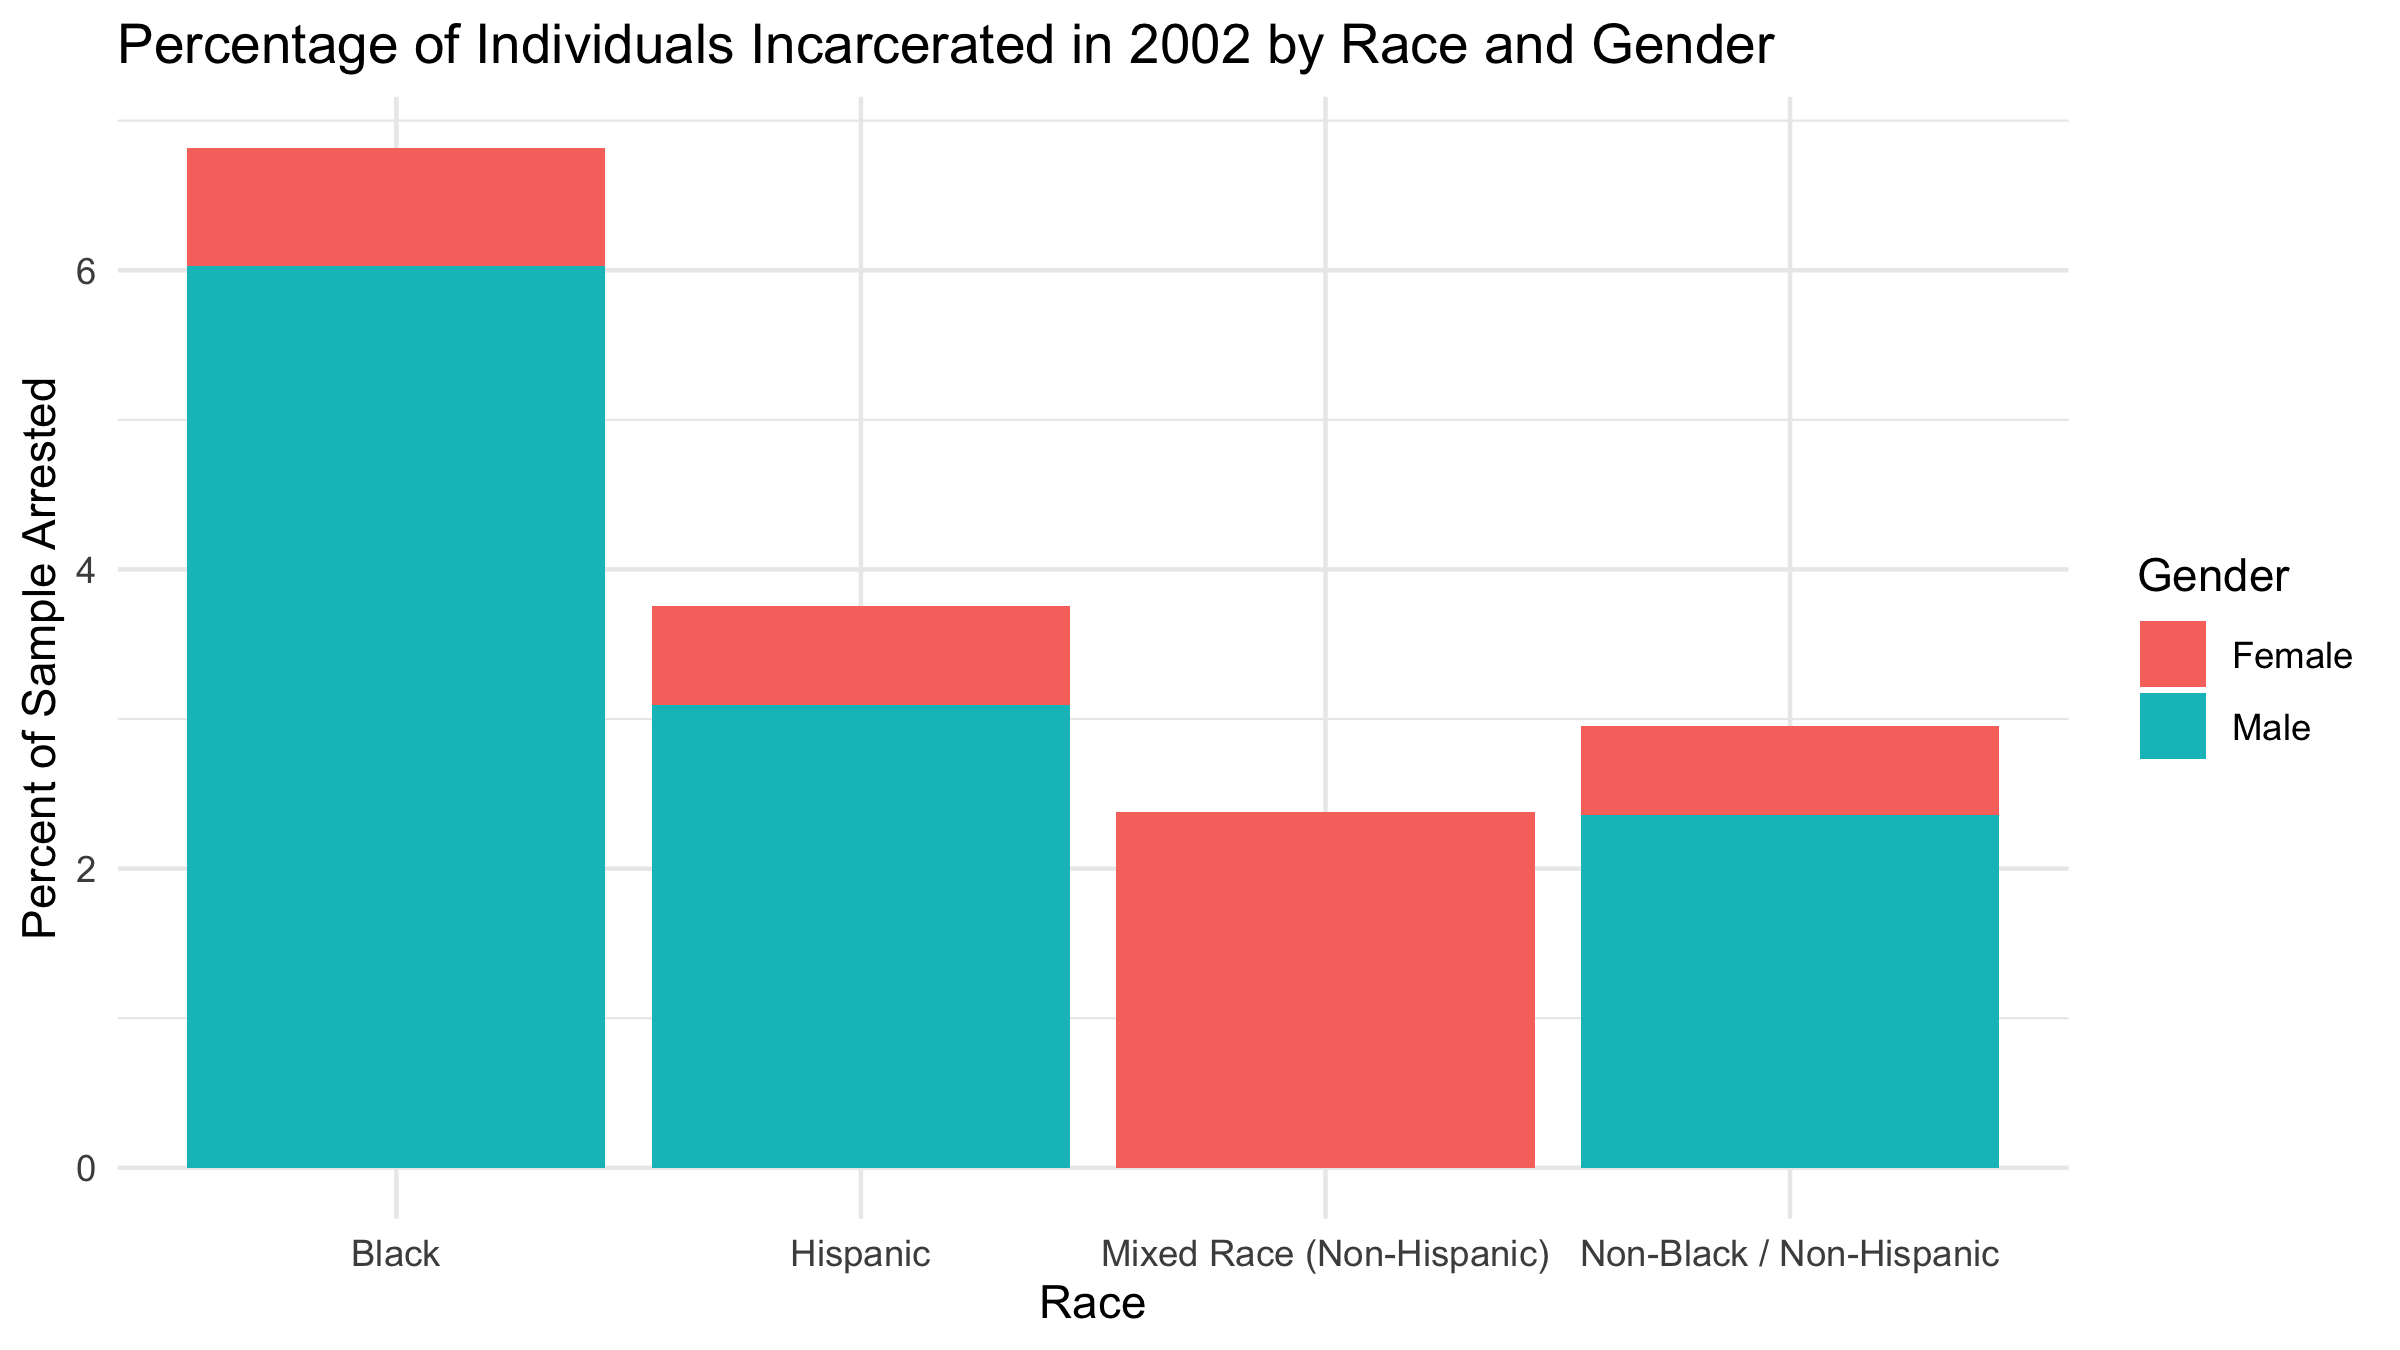
\includegraphics[width=.85\textwidth]{incarceration_by_racegender.png}
    \end{center}
    \caption{Percentage of Individuals in the Survey who were incarcerated at any point in 2002, broken down by race and gender. Mixed Race proportions should be largely ignored due to small sample size.}
    \label{fig:graph}
\end{figure}

\newpage
\section{Section 2: Table}

\begin{table}[H]

\caption{\label{tab:tab:summarystats}Percentage Incarcerated in 2002 by Race and Gender}
\centering
\begin{tabular}[t]{lrrrr}
\toprule
Gender & Black & Hispanic & Mixed Race Non Hispanic & Non Black Non Hispanic\\
\midrule
\cellcolor{gray!6}{Female} & \cellcolor{gray!6}{0.7922535} & \cellcolor{gray!6}{0.6622517} & \cellcolor{gray!6}{2.380952} & \cellcolor{gray!6}{0.5979761}\\
Male & 6.0273973 & 3.0949840 & 0.000000 & 2.3560209\\
\bottomrule
\end{tabular}
\end{table}
  
This table shows a breakdown of the percentage of the individuals in the survey that were incarcerated, broken down by \texttt{Race} and \texttt{Gender}. The percentages for the \texttt{Mixed Race (Non-Hispanic)} category because the sample size for that subcategory is so small (81 individuals, only 1 female of which was incarcerated). That aside, there is a clear trend toward men being incarcerated, with \texttt{Black Men} being almost 8 times as likely to be incarcerated as \texttt{Black Women}. Black individuals seem to be more likely to be incarcerated than other races regardless of gender.

\newpage
\section{Section 3: Regression}


% Table created by stargazer v.5.2.2 by Marek Hlavac, Harvard University. E-mail: hlavac at fas.harvard.edu
% Date and time: Thu, Feb 17, 2022 - 11:21:17
\begin{table}[!htbp] \centering 
  \caption{Regression Output. Omitted category is Black Females.} 
  \label{tab:regression} 
\begin{tabular}{@{\extracolsep{5pt}}lc} 
\\[-1.8ex]\hline 
\hline \\[-1.8ex] 
 & \multicolumn{1}{c}{\textit{Dependent variable:}} \\ 
\cline{2-2} 
\\[-1.8ex] & Likelihood of Being Incarcerated in 2002 \\ 
\hline \\[-1.8ex] 
 Hispanic & $-$0.618$^{***}$ \\ 
  & (0.209) \\ 
  & \\ 
 Mixed Race (Non-Hispanic) & $-$1.021 \\ 
  & (1.036) \\ 
  & \\ 
 Non-Black / Non-Hispanic & $-$0.866$^{***}$ \\ 
  & (0.172) \\ 
  & \\ 
 Male & 1.660$^{***}$ \\ 
  & (0.205) \\ 
  & \\ 
 Constant & $-$4.470$^{***}$ \\ 
  & (0.197) \\ 
  & \\ 
\hline \\[-1.8ex] 
Observations & 8,621 \\ 
Log Likelihood & $-$810.209 \\ 
Akaike Inf. Crit. & 1,630.419 \\ 
\hline 
\hline \\[-1.8ex] 
\textit{Note:}  & \multicolumn{1}{r}{$^{*}$p$<$0.1; $^{**}$p$<$0.05; $^{***}$p$<$0.01} \\ 
\end{tabular} 
\end{table} 

The trend from above continues in the regression table. Computed using a Logit Regression, with Incarceration Status being regressed on \texttt{Race} and \texttt{Gender}. Because the coefficients of the Log-Likelihood function are somewhat difficult to interperet (the model takes the\newline form: \(p/(1-p) = e^\beta_0 + e^\beta_1x_1\)), the magnitude of beta coefficients in the regression output may seem off. For example, the odds of a \texttt{Black Male} being incarcerated are $e^1.66 = 5.26$ times more likely than a \texttt{Black Female}. Similarly, all other races have lower odds of being incarcerated than Blacks (again mostly ignoring the Mixed Race (Non-Hispanic) category for sample-size reasons).
\end{document}
